\chapter{Bilder vom "`Innenleben"' des Detroits} \newpage\begin{landscape}

Der folgende Abschnitt zeigt Bilder, die während den Umbauarbeiten am Fahrzeug entstanden sind. Damit soll ein Blick ins Innere des Fahrzeuges gewährt werden, auch wenn dieses wieder zusammengebaut ist. Der Fokus liegt dabei auf technischen Details, wobei diese unterteilt werden in die mechanische Funktion und elektrische Komponenten.


\section{Mechanisch}
\begin{figure}[h]
	\centering
		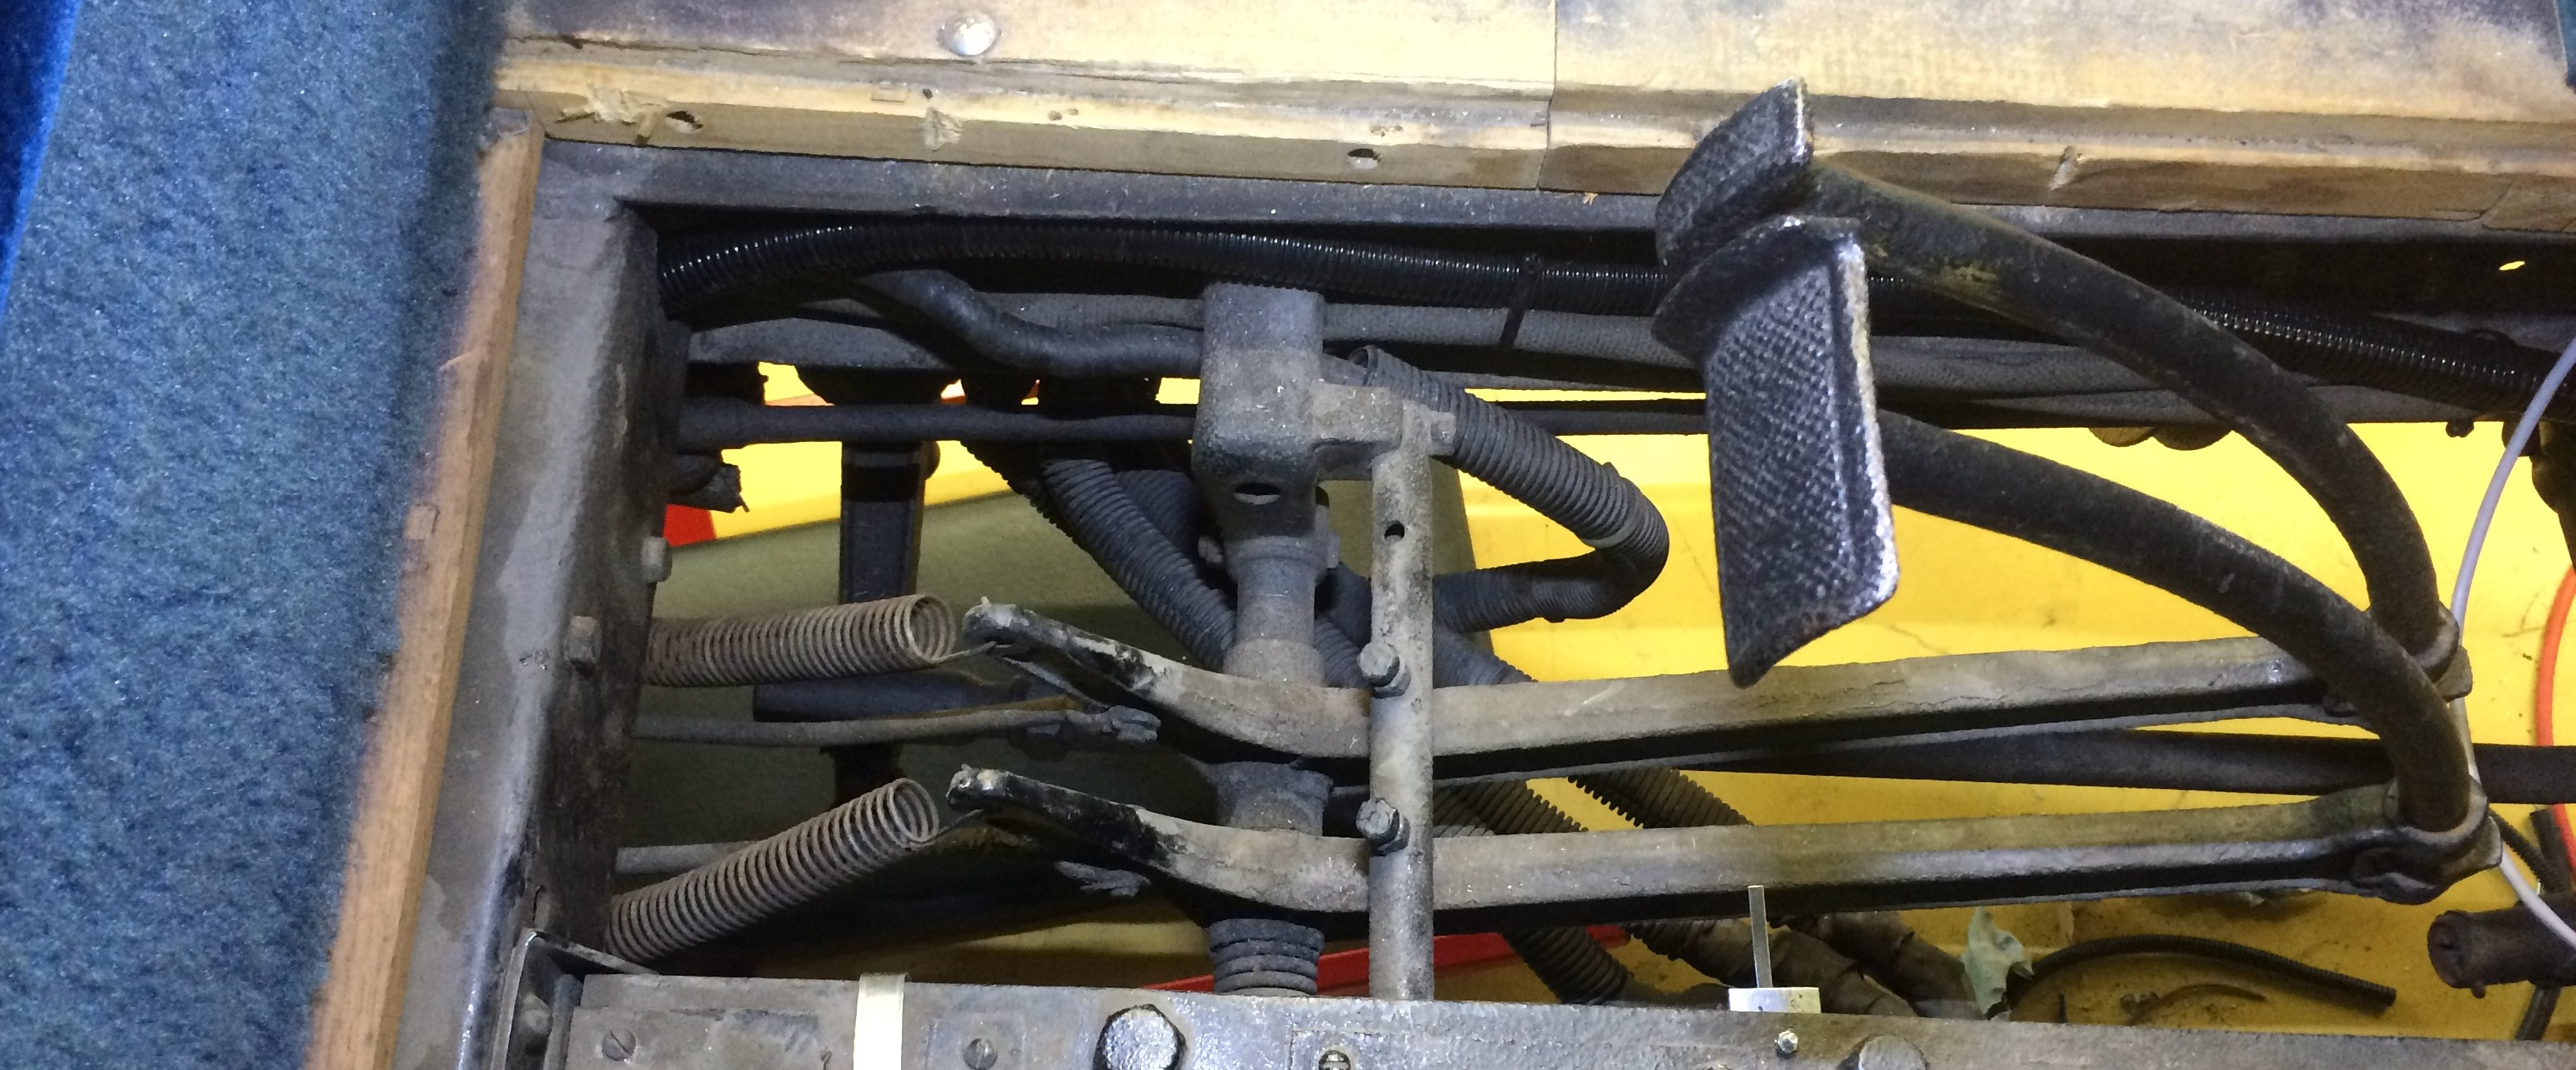
\includegraphics[width=1.30\textwidth]{images/Anhang/Bremspedale.jpg}
	\caption{Die Bremspedale mit den Federn, welche sie zurück in ihre Ausgangslage bringen}
	\label{fig:Bremspedale}
\end{figure}
\begin{figure}[h]
	\centering
		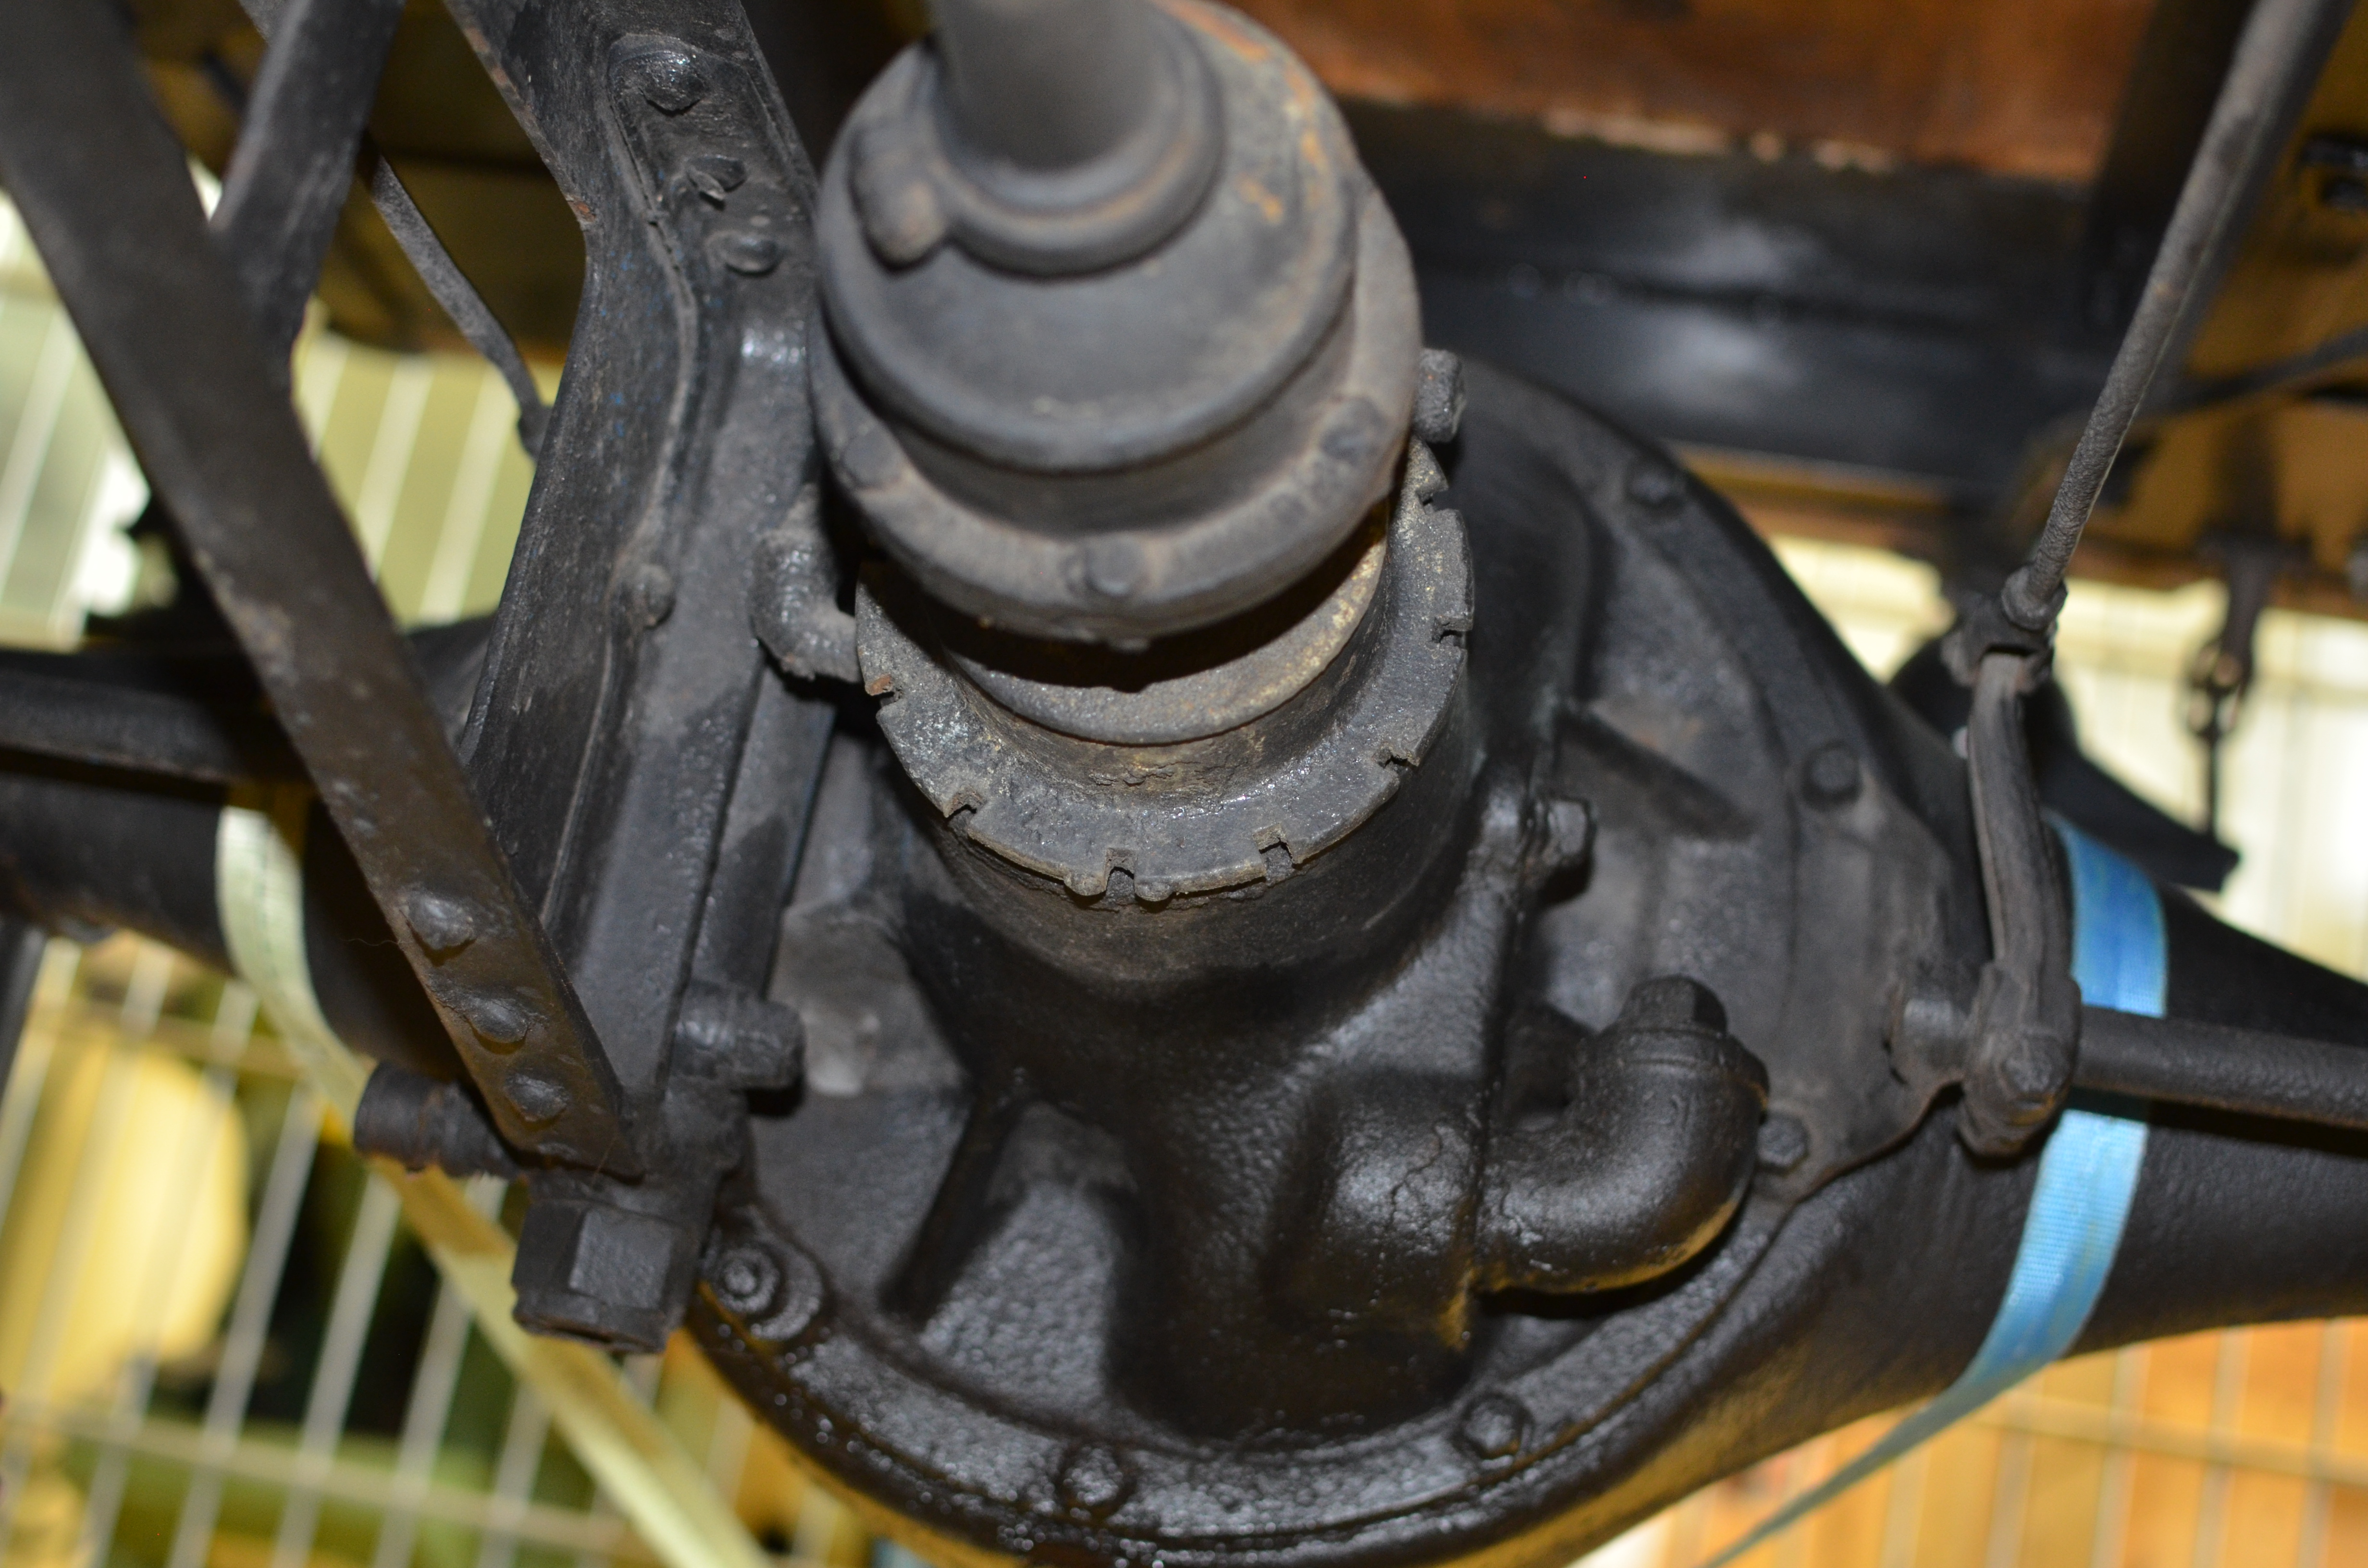
\includegraphics[width=1.30\textwidth]{images/Anhang/Differential.jpg}
	\caption{Die Welle zwischen Motor und Differential, im Hintergrund ist letzteres sichtbar}
	\label{fig:Differential}
\end{figure}
\begin{figure}[h]
	\centering
		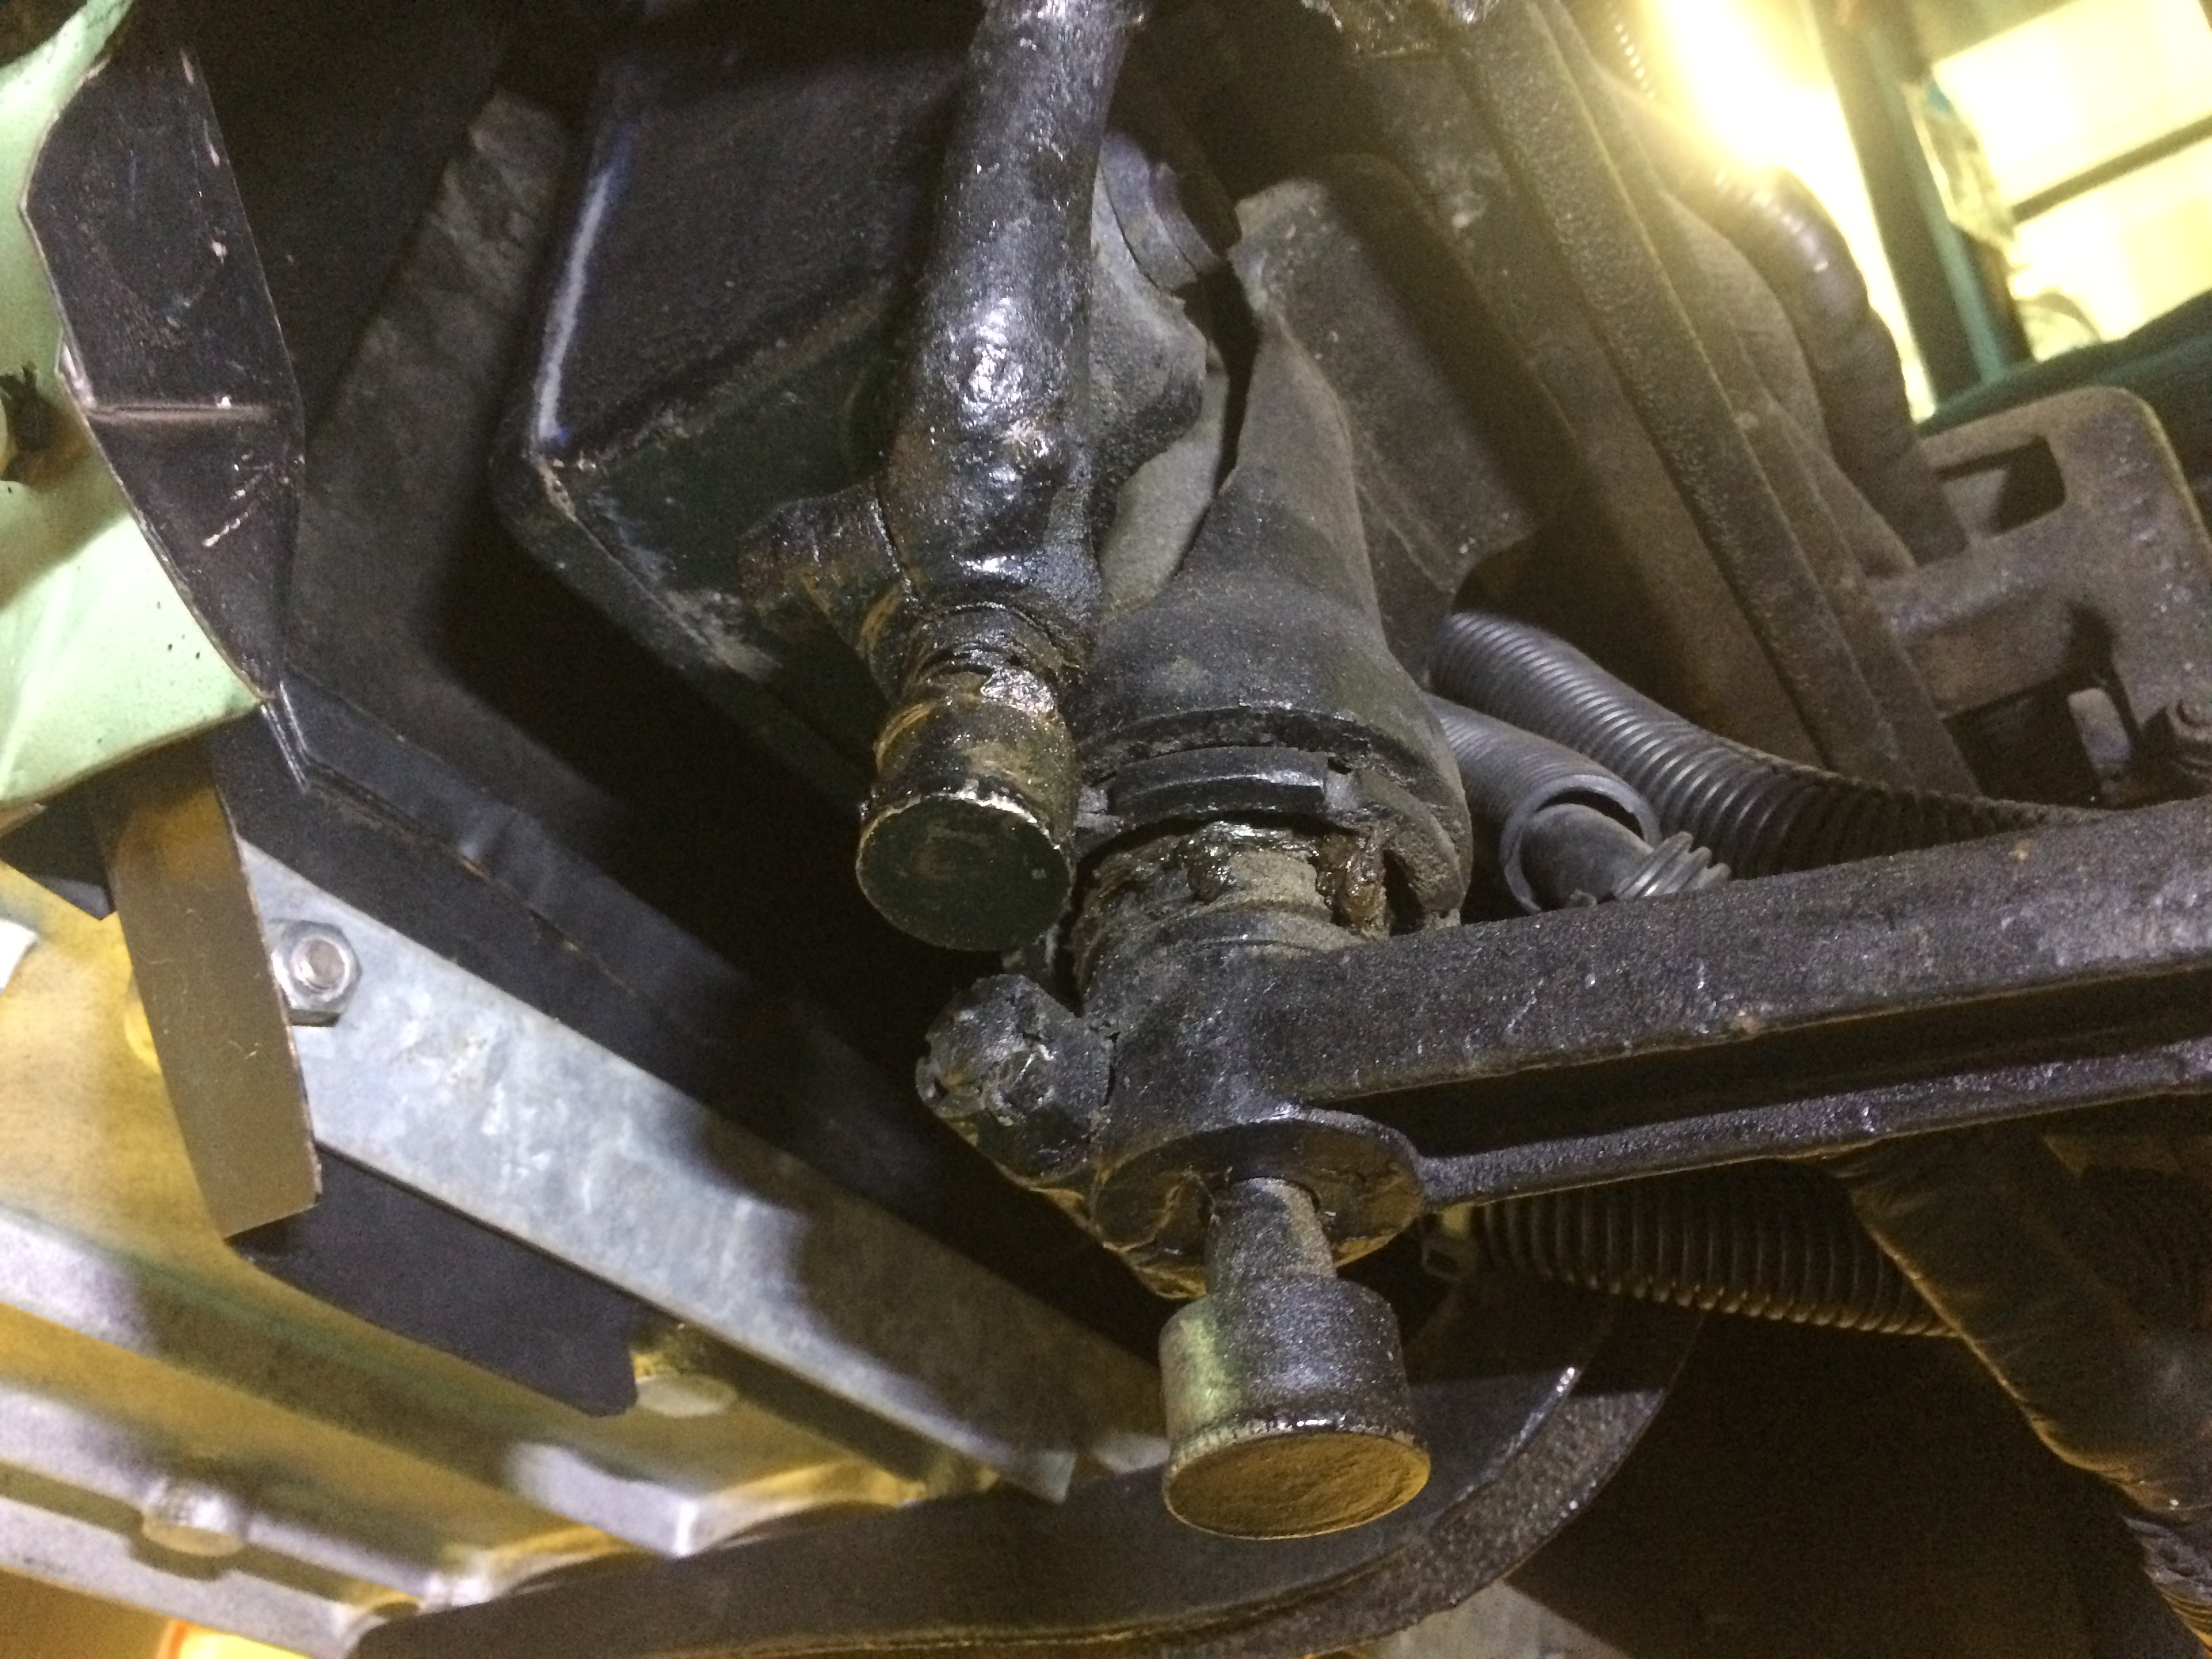
\includegraphics[width=1.30\textwidth]{images/Anhang/Lenkung_Stufenschalter.jpg}
	\caption{Die Drehbewegung von Steuerhebel und Stufenschalter werden in eine Längsbewegung umgewandelt, wobei beim Stufenschalter mit der Höhe zusätzlich noch die Fahrtrichtung gewählt wird}
	\label{fig:Lenkung_Stufenschalter}
\end{figure}
\begin{figure}[h]
	\centering
		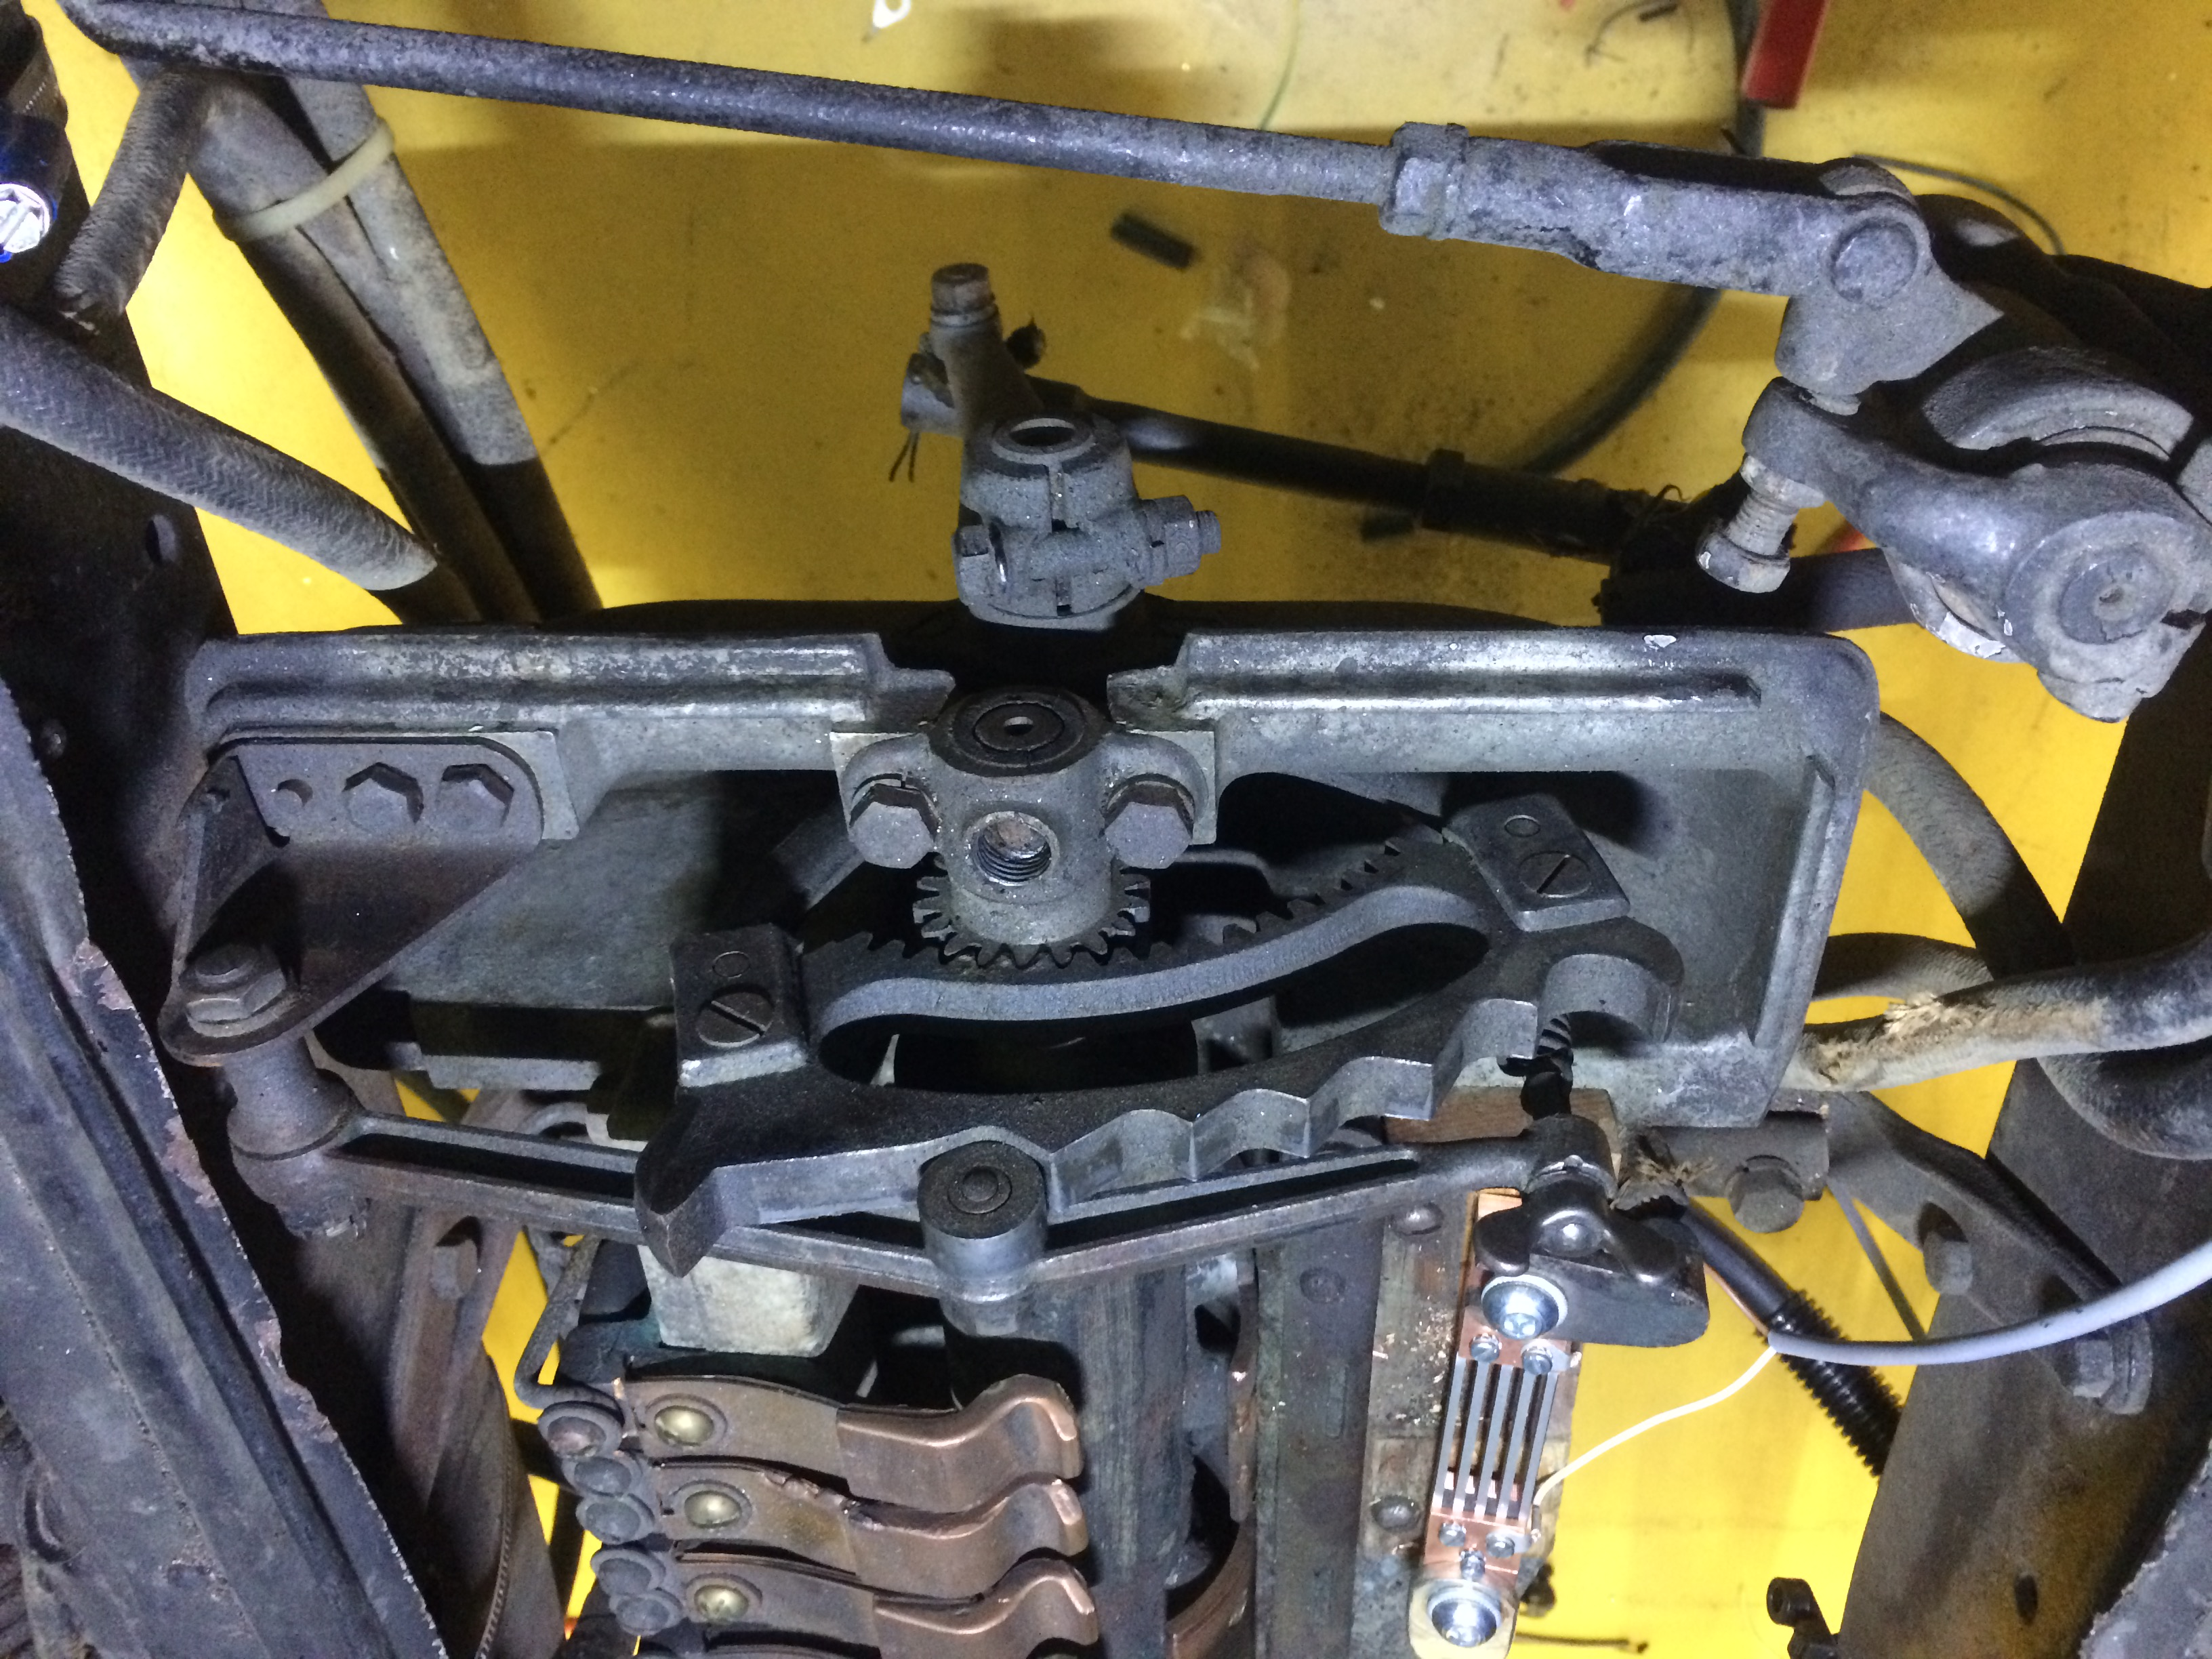
\includegraphics[angle=180,width=1.30\textwidth]{images/Anhang/Stufenschalter_2.jpg}
	\caption{Die mechanische Verriegelung der Stufen des Stufenschalters}
	\label{fig:Stufenschalter_2}
\end{figure}
\begin{figure}[h]
	\centering
		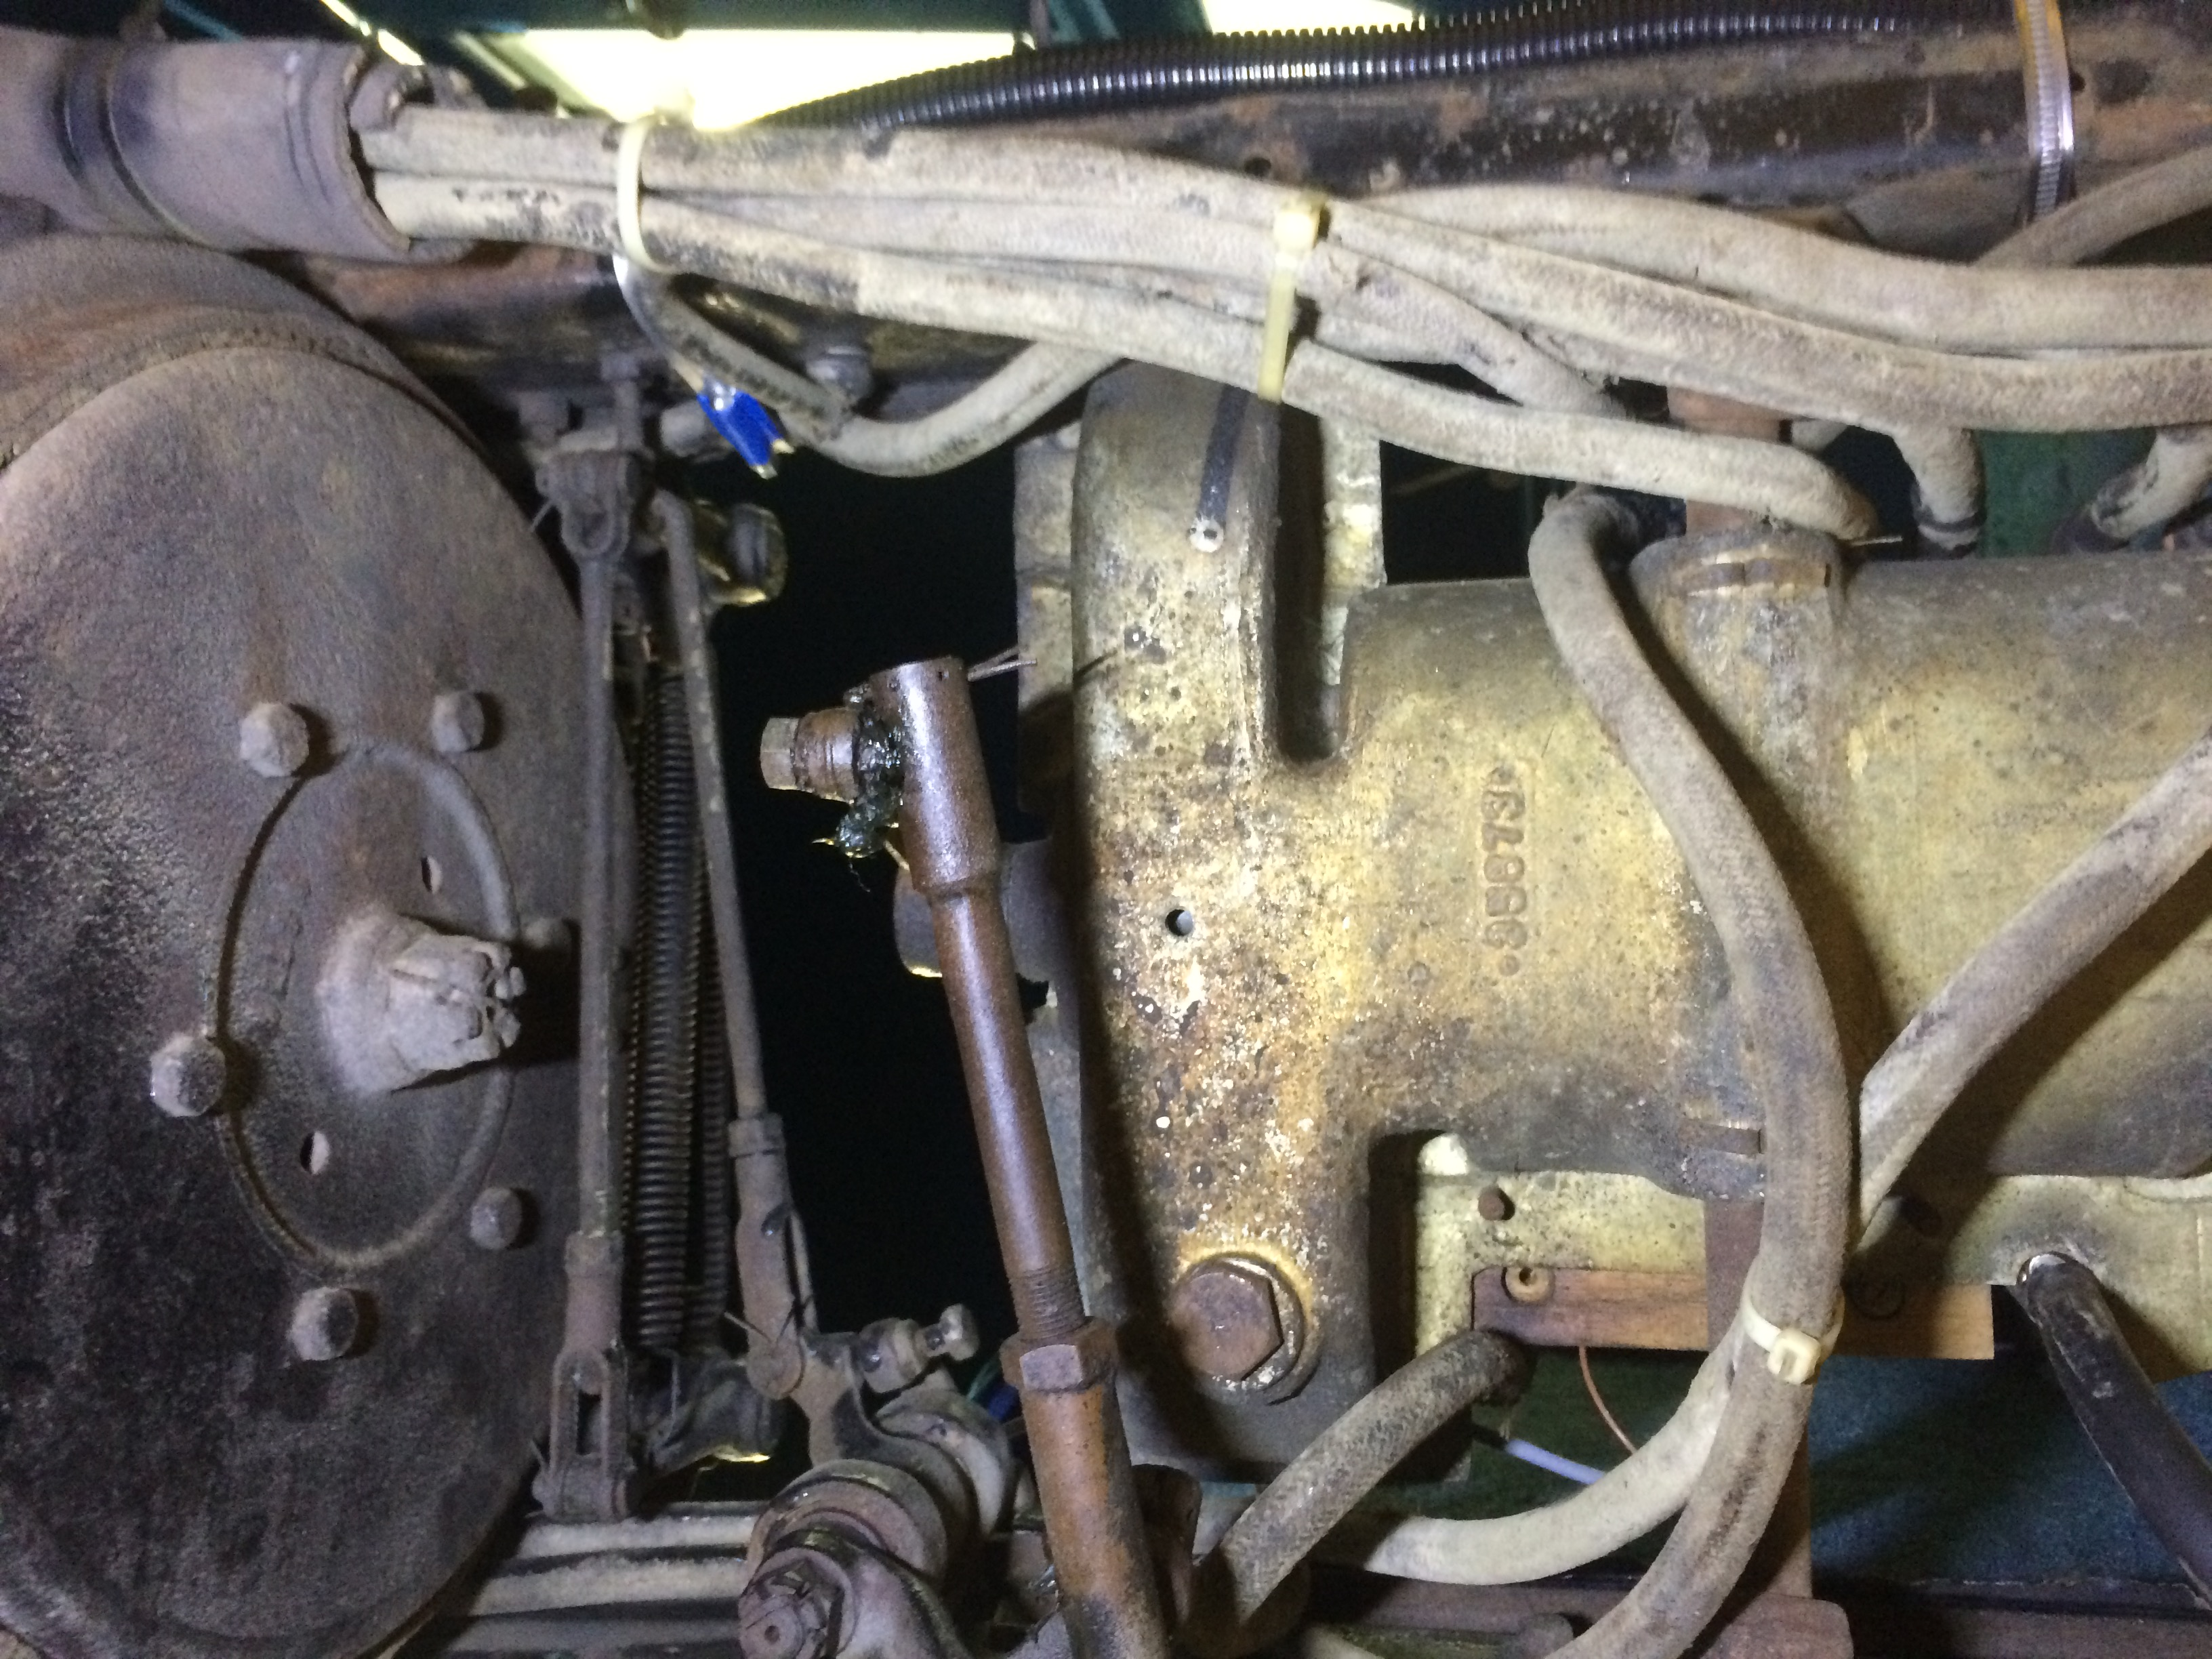
\includegraphics[angle=180,width=1.30\textwidth]{images/Anhang/Stufenschalter_1.jpg}
	\caption{Die mechanische Ansteuerung des Stufenschalters erfolgt von unten}
	\label{fig:Stufenschalter_1}
\end{figure}
\begin{figure}[h]
	\centering
		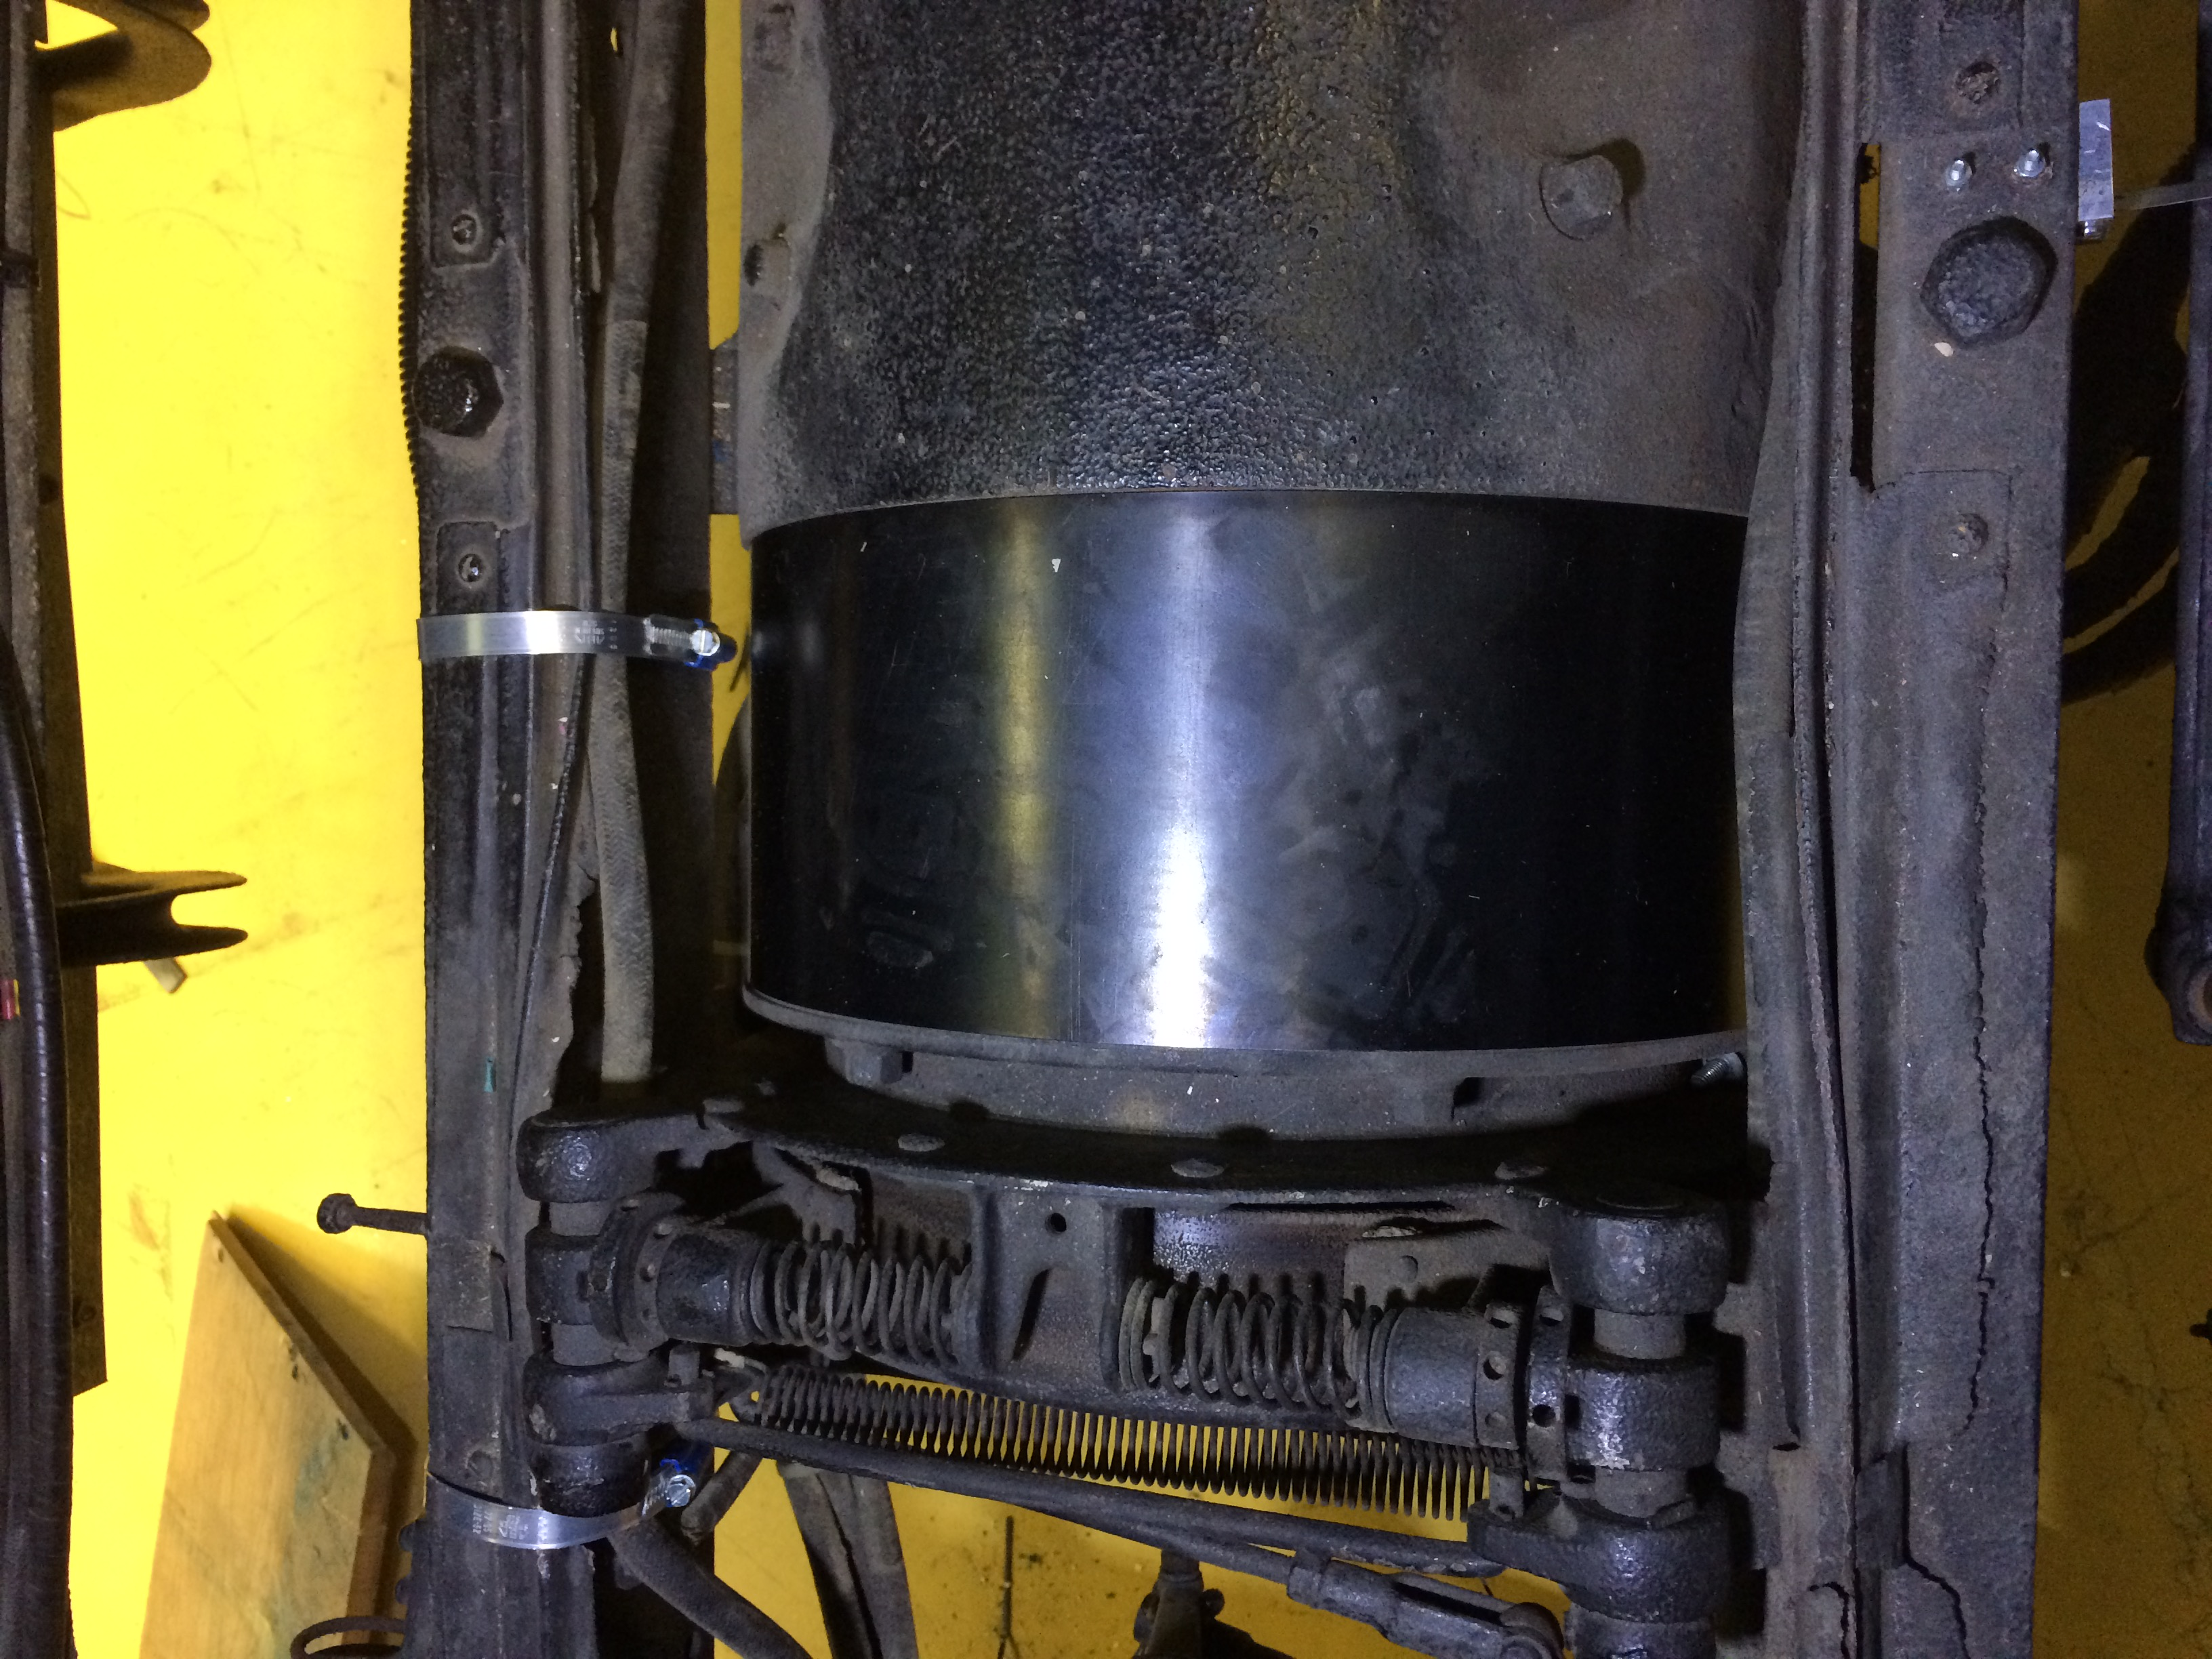
\includegraphics[angle=180,width=1.30\textwidth]{images/Anhang/Abdeckung.jpg}
	\caption{Das neue Abdeckblech für den Motor besteht aus brüniertem Stahl}
	\label{fig:Abdeckung}
\end{figure}\end{landscape}